\documentclass[allauthors,dutch]{../../cursuspresentatie}

\copyrightTim

\def\importslide#1#2{%
	\import{../../slides/tim/#1}{#2}
}

\title{\LaTeX{}-cursus Week 1}
\author{\TeX niCie}
\date{26/28 september 2022}

% Als je het bestand dumpt naar een format, worden packages hierna niet meegedumpt maar elke keer
% fris ingeladen
\csname endofdump\endcsname

\usepackage{minted} %kan later in de .cls file hierboven
\usepackage{xcolor}
\setminted[tex]{fontsize=\small, autogobble=true, linenos=true, frame=single, escapeinside=||}
\usepackage{tcolorbox}
% \usepackage{}
\definecolor{darkgreen}{rgb}{0.2,0.7,0.11}
\makeatletter
\patchcmd{\@thm}{\thm@headfont{\scshape}}{\thm@headfont{\scshape\bfseries}}{}{}
\patchcmd{\@thm}{\thm@notefont{\fontseries\mddefault\upshape}}{}{}{}
\makeatother
\newtheorem{mylemma}[]{Lemma}
\begin{document}

\section{Introduction}
\importslide{beginners}{welcome.tex}
%\importslide{beginners}{contents.tex}

\begin{frame}
	\frametitle{Agenda}

	\begin{tabular}{p{6cm} p{7cm}}
	\begin{itemize}
		\item \textcolor{blue}{Week 1} (26/28 september)
	\begin{itemize}[label=\textbullet]
		\item Introductie tot LaTeX en Overleaf
		\item LaTeX documentstructuur
		\item Tekst
		\item Wiskunde
		% \item \lang,Text formatting,Tekstopmaak,
		% \item  $ \langle $\lang,Exercises!,Oefeningen!,$ \rangle $
		% \item \lang,Structure of a document,Documentstructuur,
		% \item $ \langle $\lang,Exercises!,Oefeningen!,$ \rangle $
		% \item \lang,Formulas,Formules,
		% \item $ \mathbf\langle $\lang,Exercises!,Oefeningen!,$ \rangle $
		% \item  \lang,Images,Afbeeldingen,
		% \item $ \mathbf\langle $\lang,Exercises!,Oefeningen!,$ \rangle $
		% \item \lang,Closing remarks,Afsluitende opmerkingen,
	\end{itemize}
		\item Week 2 (3/5 oktober)
	\begin{itemize}[label=\textbullet]
		\item Referenties
		\item Afbeeldingen
		\item Extra wiskunde
	\end{itemize}
	\end{itemize}
		&
	\begin{itemize}
		\item Week 3 (10/12 oktober)
			\begin{itemize}[label=\textbullet]
			\item tabellen
			\item \textbackslash newcommand
			\item \textbackslash DeclareMathOperator
			\item bibliografie
    			\item Commutatieve diagrammen
		\end{itemize}
	\item Week 4 (17 oktober)
		\begin{itemize}
			\item Installatie Visual Studio
			\item Vragenuurtje
		\end{itemize}
	\end{itemize}
	\end{tabular}
\end{frame}

\importslide{beginners_NL}{overleaf-1.tex}
\importslide{beginners_NL}{overleaf-2.tex}

% We switchen naar Overleaf voor Live LaTeX : laat zien hoe je in kan loggen, nieuw bestand maken,
% waar de compileerknop zit en waar je tekst kan typen. ook laten zien dat er een file explorer is.

\importslide{beginners_NL}{simpledoc-1.tex}
\importslide{beginners_NL}{simpledoc-2.tex}
\importslide{beginners_NL}{simpledoc-3.tex}

% simpel document met wat tekst zoals op slide simpledoc-3 namaken. Op compileren klikken en pdf
% laten zien. laten zien wat er gebeurt als je iets fouttypt, dat er dan een error verschijnt.

\importslide{beginners_NL}{commands-1.tex}
\importslide{beginners_NL}{commands-2.tex}
\importslide{beginners_NL}{commands-3.tex}
% switch naar live LaTeX : demonstreer gebruik van de commands van zojuist. leg uit welke in de preamble gaan en 
% welke in de body.

% 5 min voor oefeningen 1 t/m 4

\begin{frame}
	\frametitle{Oefeningen}
	
	\centering
	
	%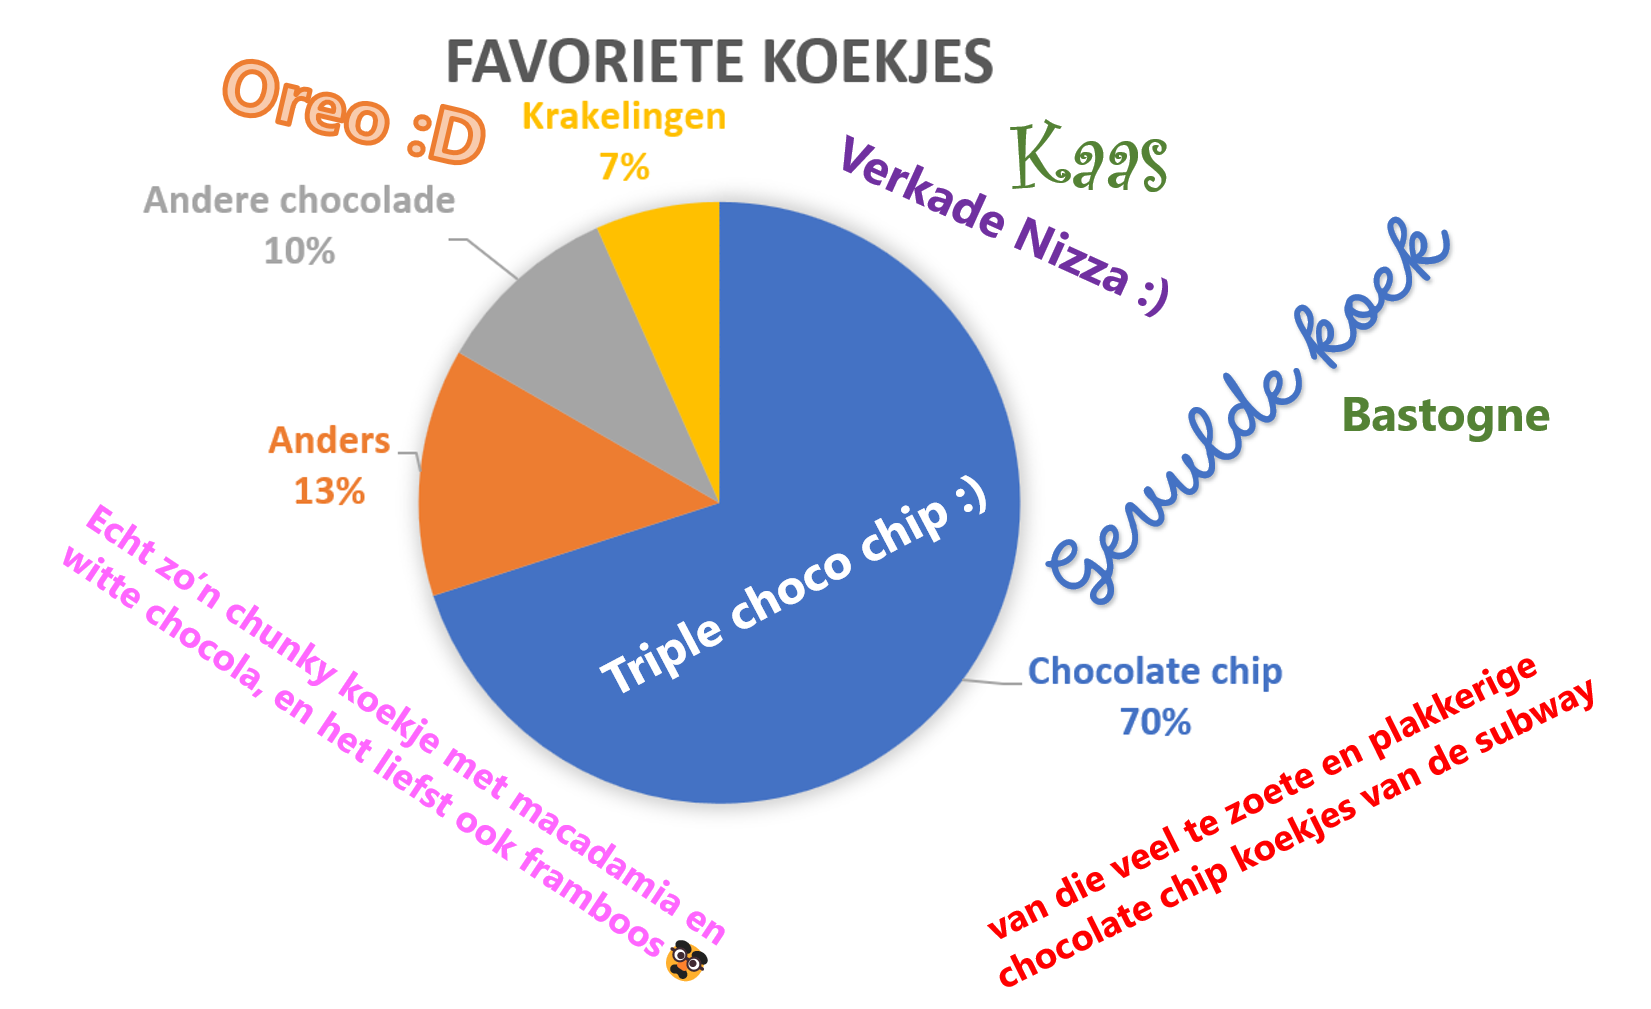
\includegraphics[width=0.9\textwidth,height=0.85\textheight,keepaspectratio]{images/cookie_art.png}
\end{frame}


\importslide{beginners_NL}{whitespace.tex}
% Vertel dat quad staat voor spazio quadratone = groot vierkant spatie en de grootte heeft van een hoofdletter M
% demo het gebruik van \ \quad en \hspace


\importslide{beginners_NL}{paragraphs-1.tex}
% maak 3 paragrafen zonder parskip. Laat zien waar de indent zit.
% leg nadruk op de witregel in LaTeX code die de paragrafen scheidt.

\importslide{beginners_NL}{paragraphs-2.tex}

% 5 min voor oefeningen 5 t/m 8

\importslide{beginners_NL}{sections.tex}

% maak 2 sections, met subsections en een subsubsection. Zet er wat tekst in. Namen van de sections:
% \section{Limieten en continuïteit}
% \subsection{De afstand in R^n}
% De norm wordt gegeven door wortel van het inproduct
% \subsubsection{Cauchy-Schwarz}
% dit is een belangrijke ongelijkheid
% \subsection{Limieten van functies}

\importslide{beginners_NL}{title.tex}

% \title{Huiswerkopdracht 2 bewijzen in de wiskunde}
% \author{Tim Weijers \and Vincent Kuhlmann}
% \date{26 september 2022}

\importslide{beginners_NL}{special-characters.tex}

% \{ f in fruit | f is een citrusvrucht \}
% 40\%, Piet \& Klaas, Dit boek kost 40\$

\importslide{beginners_NL}{format-text-1.tex}

\importslide{beginners_NL}{logical-formatting.tex}

% Dit is \textbf{vetgedrukte} tekst
% Dit is \textbf{ \textcolor{blue} blauwe vetgedrukte }} tekst

% 5 min voor oefeningen 9 t/m 11

\importslide{beginners_NL}{math-1.tex}

\importslide{beginners_NL}{math-2.tex}

% Hieruit volgt dat \( x \geq 4 \) en \( -1 \leq \sin(\theta) \leq 1 \)

\importslide{beginners_NL}{math-3.tex}

\importslide{beginners_NL}{math-4.tex}

\importslide{beginners_NL}{math-5.tex}

\importslide{beginners_NL}{math-6.tex}

\importslide{beginners_NL}{math-7.tex}

% slide met voorbeeldcode ALIGN op scherm houden. Oefeningen tot 18:55


\begin{frame}
	\frametitle{Afsluiting}
	
	De volgde cususavond is dinsdag 3 oktober en donderdag.
\end{frame}
\import{../../slides/thomas/Eerstejaars-2023}{afsluiting-1.tex}
	
\import{../../slides/misc/}{misc-license.tex}

\end{document}
